% !TEX root = base.tex 


\chapter{Hematite Film Growth on Single Crystal Substrates}
\label{ch:single.crystal.growth}


\chintro{This section describes the results for studies of \ce{Fe2O3} film growth on
single crystal substrates. Film orientation and phase determination was carried out using
electron backscatter diffraction analysis and x-ray diffraction. Films were grown on
\ce{Al2O3} (0001), \ce{SrTiO3} (111), and \ce{SrTiO3} (001) substrates. The films were
epitaxial on \ce{Al2O3} and \ce{SrTiO3} (111). The films on \ce{SrTiO3} (001) were
polycrystalline, but show significant texture. Film grains on these substrates fall into
five distinct groupings. The orientation relationship between substrate and film for each
orientation group was determined.}


\section{Film Growth on Strontium Titanate (111) Substrates}
\label{sec:single.growth.111}


\figureref{111maps} shows \abbr{EBSD} maps of a film grown on \ce{SrTiO3} (111) substrate. 
\begin{figure}
	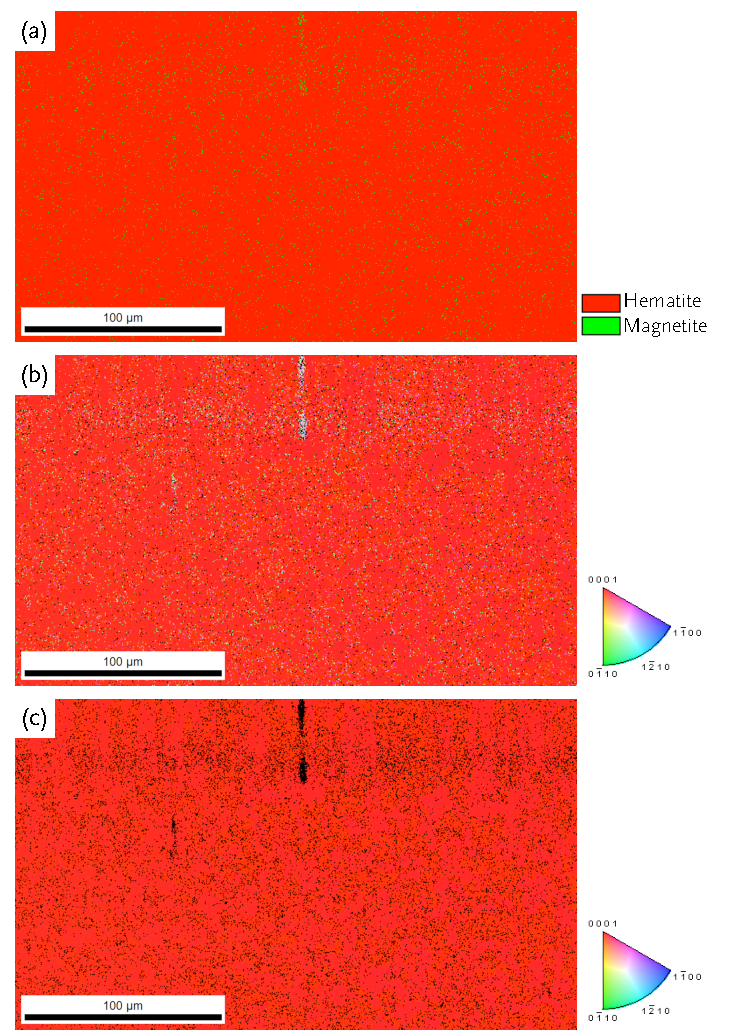
\includegraphics[width=\textwidth]{111maps.pdf}
	\caption[\abbr{EBSD} maps for film on \ce{SrTiO3} (111)]{%
		(a) \abbr{EBSD} phase map for an \ce{Fe2O3} film on \ce{SrTiO3} 
		(111). Red points represent hematite grains and green points 
		represent magnetite. (b) An inverse pole map of the same area 
		of the sample, showing only hematite grains. (c) The selection 
		of points used for the generation of pole figures.}
	\label{fig:111maps}
\end{figure}
\figureref{111maps}(a) is a phase map of all recorded points in the scan. During the
automated scan, the \abbr{EBSD} software was allowed to assign either magnetite or hematite phase
for each recorded pattern. In this map, points indexed as hematite phase appear red, while
points indexed as magnetite are green. The red points (hematite) comprise 97.5 percent of
the total data, while only 2.5 percent of points were indexed as magnetite (green).
Additionally, the points indexed as magnetite don't appear in any perceivable pattern.
Instead, they appear to be distributed randomly over the scan area. These two facts
together suggest that the magnetite points can be attributed to errors in the EBSD
process, such as poor pattern quality, surface contamination, or areas of poor film
quality, such as the macroscopic particles resulting from the pulsed laser deposition
process. Within the experimental limit, the film is considered to be comprised of solely
hematite phase. 

\figureref{111maps}(b) depicts an inverse pole map of the same dataset, with the exception
that all magnetite points (green in \figureref{111maps}(a)) have been removed from the
set. An inverse pole map depicts the crystallographic direction normal to the sample
surface at each measured point. A color gradient is assigned to the stereographic unit
triangle, which through symmetry represents all possible surface orientations for a given
crystal system. Each point in the inverse pole map is colored according to its surface
normal's position in the crystallographic triangle. A point with a surface normal of
(0001) would appear as red on this map, while a point with (1\={1}00) appears as blue. The
majority of points in this scan lie near the (0001) orientation, appearing red on the map.
The remaining points are randomly distributed across the surface and in orientation space.
As a result, the same factors that result in magnetite points are assumed to be
responsible for these points on the inverse pole map. Even if this attribution is
incorrect, and small portions of magnetite phase or non-epitaxial hematite exist in the
film, a large majority of the points were indexed as hematite. Further optimization of the
deposition parameters could improve film quality and reduce these undesired portions.
\figureref{111maps}(c) depicts in inverse pole map containing only the points within
15\si{\degree} the (0001) orientation. This data was used to generate the following pole
figures for analysis of film/substrate orientation relationships.

%\sidefigure[Pole figures for the data represented in \figureref{111maps}]{%
%	Pole figures for the data represented in \figureref{111maps}. 
%	(a) (0001) reflection showing c-axis out of plane. (b) (10\={1}0) 
%	reflection showing 6-fold symmetry in the plane. (c) (1\={2}10) 
%	reflection showing 6-fold symmetry in the plane.
%	\label{fig:111polefigures}
%	}{%
%	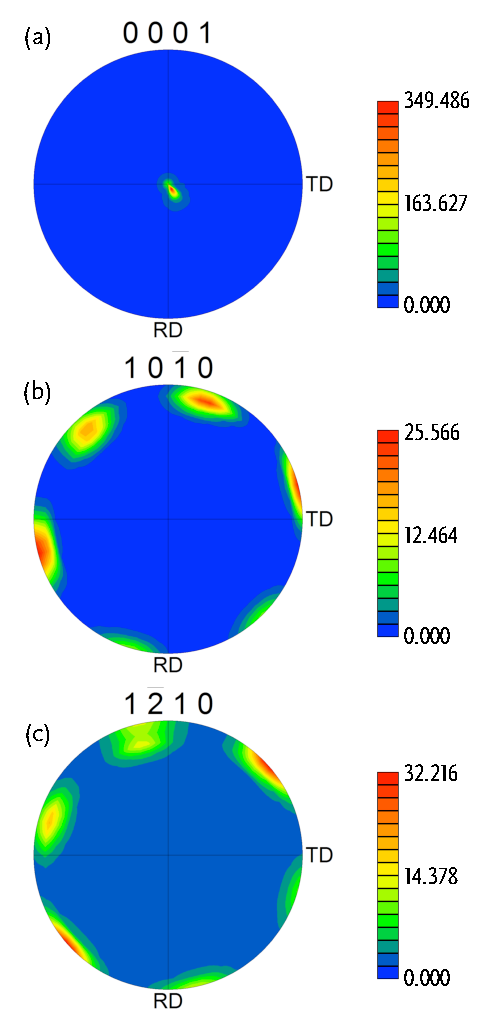
\includegraphics[width=\marginparwidth]{111polefigures.pdf}
%}{-8}
\begin{figure}
	\centerline{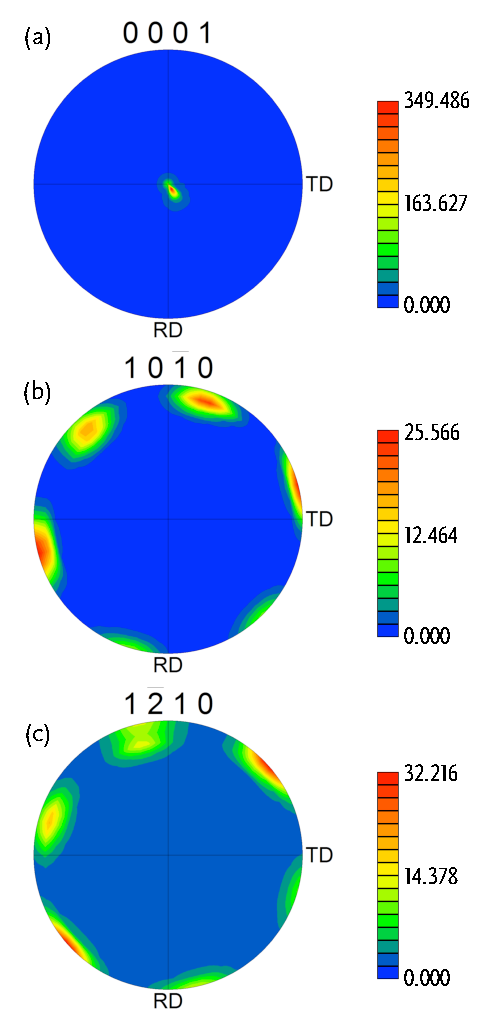
\includegraphics[width=0.5\textwidth]{111polefigures.pdf}}
		\caption[Pole figures for the data represented in \figureref{111maps}]{%
			Pole figures for the data represented in \figureref{111maps}. 
	(a) (0001) reflection showing c-axis out of plane. (b) (10\={1}0) 
	reflection showing 6-fold symmetry in the plane. (c) (1\={2}10) 
	reflection showing 6-fold symmetry in the plane.}
	\label{fig:111polefigures}
\end{figure}
Pole figures represent a distribution of specific crystal orientations in the reference
frame of the sample. The center of the pole figure represents the direction normal to the
sample surface. Points on the edges are directions in the plane of the sample. A
crystallographic plane is chosen, and the distribution of that direction in space is
plotted on the pole figure. A color gradient is used to depict which directions in the
sample reference frame that crystallographic plane normal is most prevalent. For the data
plotted in \figureref{111polefigures}, red represents sample directions with high
population of the chosen crystal orientation. Blue represents sample directions with a low
population. Units on pole figures are multiples of random density (\abbr{MRD}), 
representing the texture of the examined sample compared to that of an untextured sample. 
These pole figures allow for the examination of both in plane and out of plane
crystal orientation relationships. For all pole figures presented in this document,
texture calculations were performed using the built in discrete binning method with a bin
size of \SI{5.0}{\degree}.

\figureref{111polefigures}(a) is the pole figure for the (0001) plane (the hexagonal
c-axis). As might be guessed from the inverse pole maps, the (0001) zone is only found
directly out of plane of the sample. From this, the out of plane orientation can be
determined to be \ce{Fe2O3}(0001)||\ce{SrTiO3}(111). Figures \ref{fig:111polefigures}(b)
and \ref{fig:111polefigures}(c) are pole figure for (10\={1}0) and (1\={2}10) planes
(prismatic directions in the hexagonal unit cell, orthogonal to the c-axis). These pole
figures show that the prismatic directions are parallel to the sample surface. They also
show 6-fold  symmetry. This suggests that the in a-axis directions are preferentially
lining up with specific substrate directions. In this work, the orientation of the sample
in the \abbr{EBSD} chamber was not tracked. It is not known which direction the <1\={1}0>
substrate directions lie in the sample reference frame. The 6-fold symmetry suggests the
<1\={1}0> family of substrate directions as a likely candidate for determining the in
plane orientation of the \ce{Fe2O3} film. The set of substrate <1\={1}0> directions that
lie in the (111) plane shows 6-fold symmetry around the [111] direction. A comparison of
the lattice parameters for the film and substrate gives further support to this
hypothesis. The lattice parameter for the a-axis of \ce{Fe2O3} is \SI{5.035}{\angstrom}.
The length of the <1\={1}0> direction in the cubic substrate is \SI{5.225}{\angstrom}.
This gives a lattice mismatch of 3.8\%. From this analysis, it is proposed that the
in-plane orientation relationship for \ce{Fe2O3} films on \ce{SrTiO3} (111) substrates is
\ce{Fe2O3}[100]||\ce{SrTiO3}[1\={1}0]. 

The pole figures presented in \figureref{111polefigures} have allowed for the
determination of the orientation relationship for epitaxial films of \ce{Fe2O3} on
\ce{SrTiO3} substrates. It is determined that for the out of plane relationship,
\ce{Fe2O3}(0001)||\ce{SrTiO3}(111). For the in plane relationship,
\ce{Fe2O3}[100]||\ce{SrTiO3}[1\={1}0].


\section{Film Growth on Strontium Titanate (001) Substrates}
\label{sec:single.growth.001}


\subsection{\abbr{EBSD} Mapping}
\label{subsec:single.growth.mapping}


\ce{Fe2O3} film growth on \ce{SrTiO3}(001) substrates is significantly more complicated
than growth on \ce{SrTiO3}(111) substrates. X-ray diffraction immediately shows that films
on \ce{SrTiO3}(001) are not singly-textured. Multiple film peaks appear in the
\texttheta-2\texttheta{} scan of the \ce{Fe2O3} film on \ce{SrTiO3}(001) shown in
\figureref{001xray}. 
\begin{figure}
\centering
	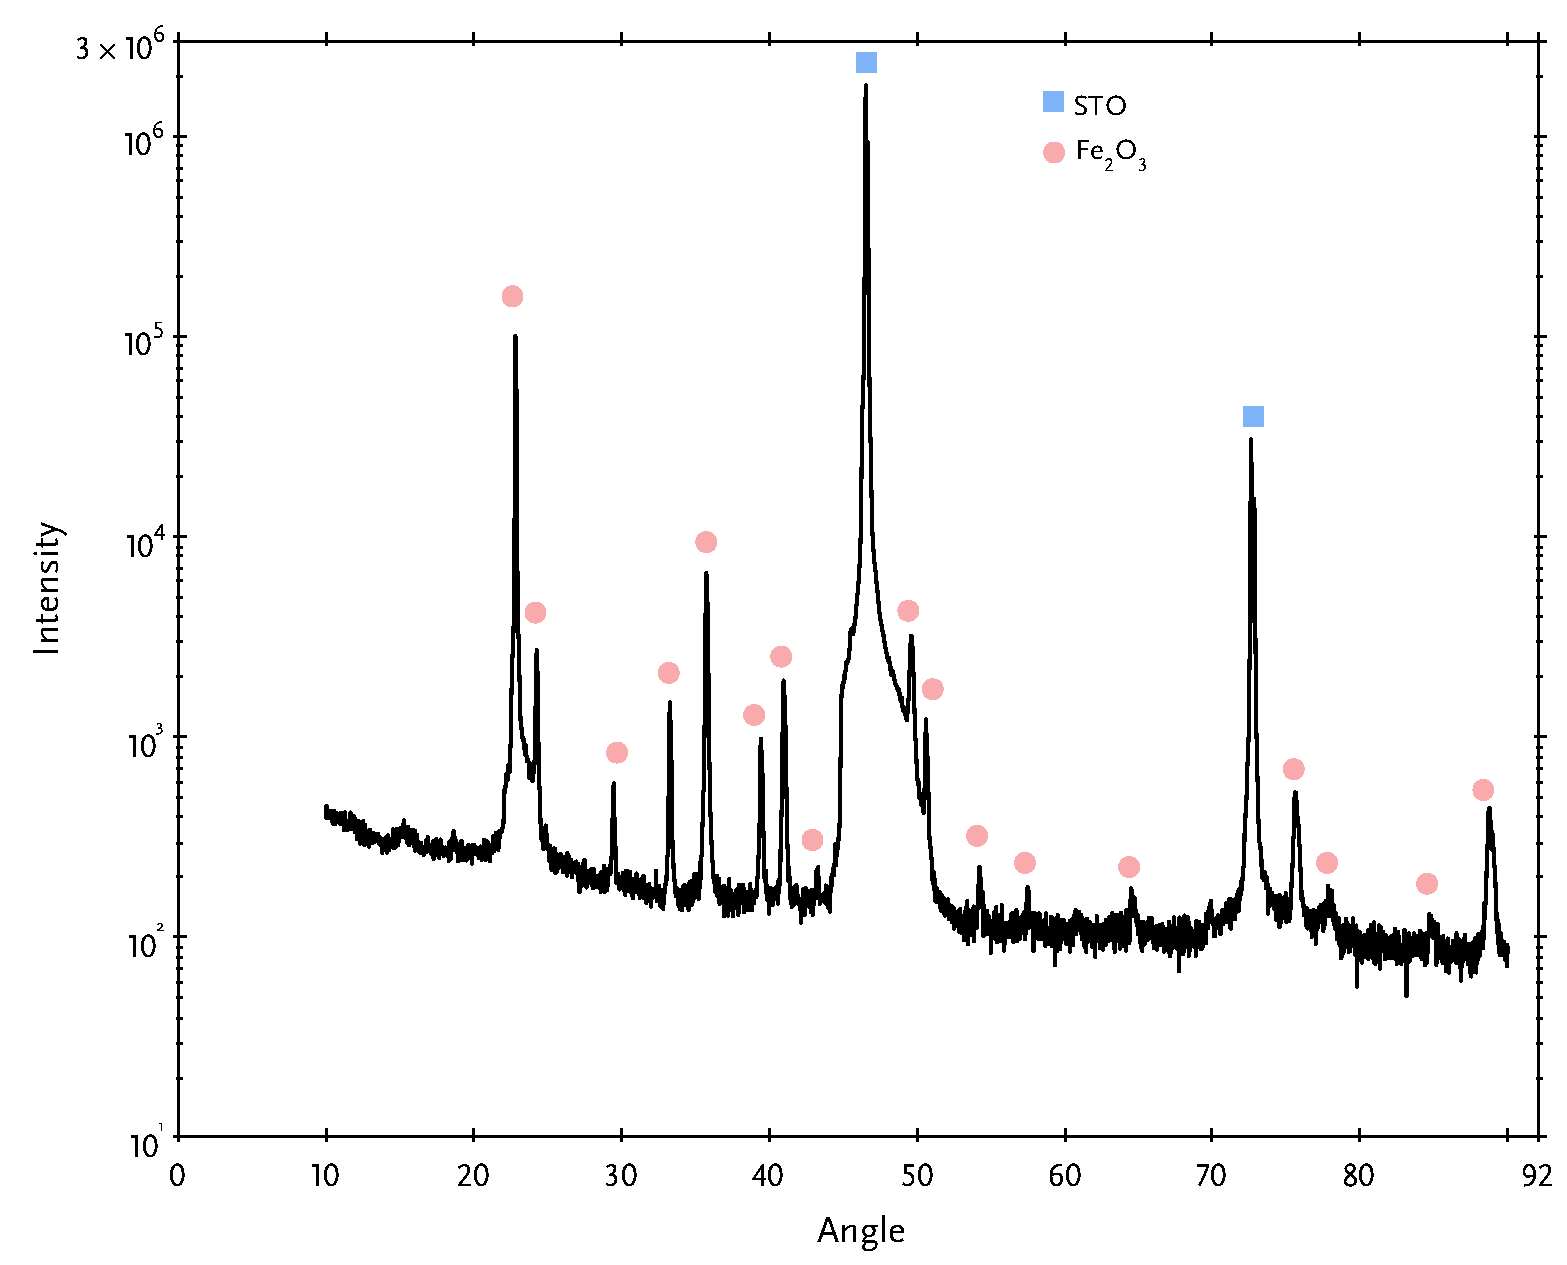
\includegraphics[width=0.8\textwidth]{001xray.pdf}
	\caption[\abbr{XRD} pattern for \ce{Fe2O3} film on \ce{SrTiO3}]{%
		X-ray diffraction pattern for \ce{Fe2O3} film grown on 
		\ce{SrTiO3} (001) substrate. Points marked with a blue 
		square are substrate peaks. Points marked with a red 
		circle are film peaks.}
	\label{fig:001xray}
\end{figure}
After initial X-ray analysis, the film was examined using electron backscatter
diffraction. \figureref{001map} shows an inverse pole map of the as \abbr{EBSD} data. While
scanning the film, the \abbr{EBSD} software was once again allowed to index each film point as
either hematite, magnetite, or strontium titanate. The map in \figureref{001map} only
shows points indexed as hematite. 
\begin{figure}
	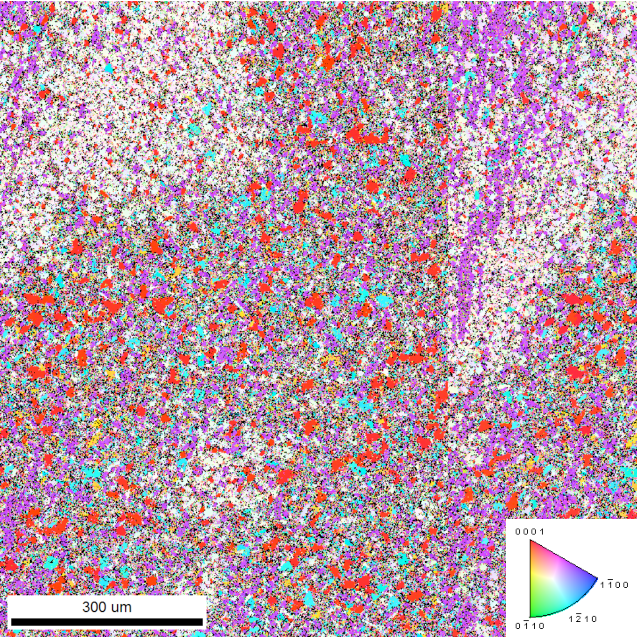
\includegraphics[width=\textwidth]{001map.pdf}
	\caption[\abbr{EBSD} map of \ce{Fe2O3} film on \ce{SrTiO3} (001)]{%
		Inverse pole \abbr{EBSD} map of an \ce{Fe2O3} film on \ce{SrTiO3} (001) 
		substrate. Five distinct color bins, labeled red, purple, white, 
		cyan, and yellow, are observed.}
	\label{fig:001map}
\end{figure}
Points indexed as either of the other two possible phases appear black on the map. It is
noted that the majority of the points in the scan area indexed as hematite, indicating
that the film was hematite phase \ce{Fe2O3}, and that the collected diffraction patterns
were from the film, not the substrate. It is apparent that the texture of the film on
\ce{SrTiO3}(001) is not random. The inverse pole map shows grains falling into five
distinct color bins. These bins will be referred to as red, cyan, purple, white, and
yellow. Table \ref{tab:sto001summary} lists the fraction of points in the scan that make
up each color bin. 

\begin{table}
  \centering 
  \begin{tabular}{lrr}
	
  		 &  
		\multicolumn{1}{c}{Number} & 
		\multicolumn{1}{c}{Area}   \\
		
		&  
		\multicolumn{1}{c}{of Points} & 
		\multicolumn{1}{c}{Fraction}   \\


		\cmidrule(lr){2-2}
    	\cmidrule(lr){3-3}
	
   		Red & 
		45,072 & 
		0.105 \\
		
		Cyan & 
		37,497 & 
		0.088 \\
		
		Purple & 
		55,640 & 
		0.130 \\
		
		White & 
		103,881 & 
		0.244 \\
		
		Yellow & 
		14,914 & 
		0.035 \\
		
		\textsc{all data} & 
		425,917 & 
		1.000 \\

	\end{tabular}
  	\caption[Summary of color area fractions from \figureref{001map}]{%
	Summary of the area fraction of points falling into the 
	five color bins from the map in \figureref{001map}. The total number of points falling
into one of the five color bins is 257,004, representing a 60.4\% fraction of the total
number of points.}
	\label{tab:sto001summary}
\end{table}

%\sidetable[Summary of color area fractions from \figureref{001map}]{%
%	Summary of the area fraction of points falling into the 
%	five color bins from the map in \figureref{001map}.
%	\label{tab:sto001summary}}{%
%  	\vspace{-3.5in}
%	\begin{tabular}{lrr}
%	
%  		 &  
%		\multicolumn{1}{c}{Number} & 
%		\multicolumn{1}{c}{Area}   \\
%		
%		&  
%		\multicolumn{1}{c}{of Points} & 
%		\multicolumn{1}{c}{Fraction}   \\
%
%
%		\cmidrule(lr){2-2}
%    	\cmidrule(lr){3-3}
%	
%   		Red & 
%		45,072 & 
%		0.087 \\
%		
%		Cyan & 
%		37,497 & 
%		0.096 \\
%		
%		Purple & 
%		55,640 & 
%		0.108 \\
%		
%		White & 
%		103,881 & 
%		0.202 \\
%		
%		Yellow & 
%		14,914 & 
%		0.029 \\
%		
%		\textsc{all data} & 
%		513,205 & 
%		1.000 \\
%
%	\end{tabular}
%}
The fractions do not add up to 1, as the color bins do not include any of the black points
in the map, nor the points on the map falling outside these color bins. When the entire
scan area is shown, outlying points are not visible on the map. When zoomed in, individual
outlier points are clearly visible, and account for the points not used in calculating the
following pole figures. The total area fraction represented on this map represents a 
majority (60.4\%) of the collected points. This proportion of points is similar to the number of
points obtained if the entire dataset is partitioned to only include points with a confidence
index greater than 0.1 (compared to a mean value of 0.18). That partition includes all the color
bins here, though it is important to note that partitioning via confidence index was not
used to create the actual datasets. It is pointed out only to support that the population of
points used in the following calculations likely correspond to high quality measurements.



\begin{figure}
\begin{center}
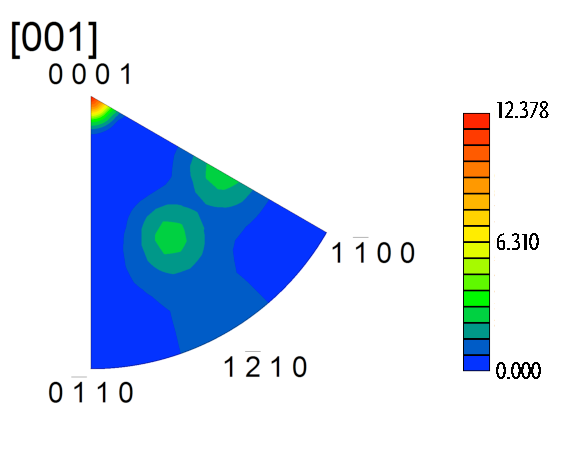
\includegraphics[width=0.5\textwidth]{allpointsipf.pdf}
\caption[Inverse pole figure of dataset represented in \figureref{001map}]{%
	Inverse pole figure of the entire dataset represented in \figureref{001map}.}
\label{fig:allpointsipf}
\end{center}
\end{figure}
%\sidefigure[Inverse pole figure of dataset represented in \figureref{001map}]{%
%	Inverse pole figure of the entire dataset represented in \figureref{001map}.
%	\label{fig:allpointsipf}
%	}{%
%	 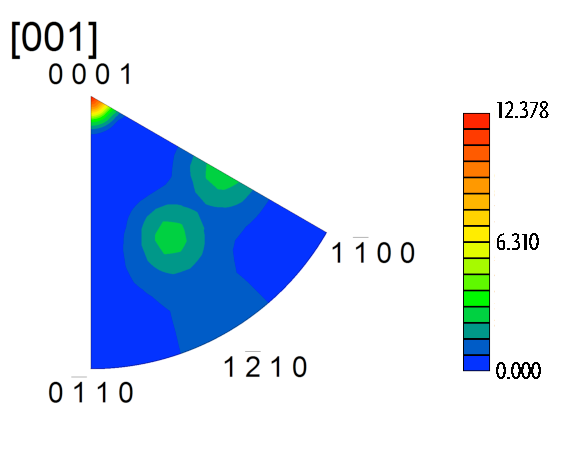
\includegraphics[width=\marginparwidth]{allpointsipf.pdf}
%}{-5}
\figureref{allpointsipf} is an inverse pole figure of the points on the map in
\figureref{001map}. Similar to the pole figures presented earlier, inverse pole shows the
distribution of crystallographic directions normal to the sample surface in the crystal
reference frame. While the pole figure shows the distribution of a given crystallographic
direction in the sample reference frame, the inverse pole figure shows the distribution of
all crystallographic directions in a given sample direction. In this case, the figure
shows the distribution of crystallographic directions that lie in the sample normal
direction. Once again, red represents areas of high population, while blue represents
areas of low population. Five distinct maxima are observed, correlating with each of the
colors observed on the inverse pole map. Each maximum occurs at a low index plane. Table
\ref{tab:orientationsummary} summarizes the crystal direction corresponding to each color
bin.
\begin{table}
	\centering 
	\begin{tabular}{lrc}

		&  
		\multicolumn{1}{c}{Orientation}  \\
		
		\cmidrule(lr){2-2}

   		Red & 
		(0001)    \\
		
		Cyan & 
		(1\={2}10)   \\
		
		Purple & 
		(10\={1}2) \\
		
		White & 
		(1\={2}13) \\
		
		Yellow & 
		(0\={1}14) \\
		
	\end{tabular}
	\caption[Summary of Miller indices]{%
	Miller indices for the orientation represented by each of 
	the color bins seen in the inverse pole map in \figureref{001map}.}
	\label{tab:orientationsummary}
\end{table}
%\sidetable[Summary of Miller indices]{%
%	Miller indices for the orientation represented by each of 
%	the color bins seen in the inverse pole map in \figureref{001map}.
%	\label{tab:orientationsummary}}{%
%	\vspace{-1.5in} %to move the table
%	
%    \begin{tabular}{lrc}
%
%		&  
%		\multicolumn{1}{c}{Orientation}  \\
%		
%		\cmidrule(lr){2-2}
%
%   		Red & 
%		(0001)    \\
%		
%		Cyan & 
%		(1\={2}10)   \\
%		
%		Purple & 
%		(10\={1}2) \\
%		
%		White & 
%		(1\={2}10) \\
%		
%		Yellow & 
%		(0\={1}14) \\
%		
%	\end{tabular}
%}
These zones represent the planes that will be analyzed using pole figures.

The data was manually partitioned into subsets corresponding to  each color bin. This
allows for texture analysis of each set of orientations independent of the other sets.
This is a distinct advantage of using the \abbr{EBSD} technique over x-ray diffraction pole
figure analysis. Unlike X-ray diffraction, which examines the entire scan area
simultaneously,  \abbr{EBSD} ties each piece of orientation data back to a location on the
sample. After measurement, data can be partitioned and manipulated; subsets of data can be
extracted for further analysis. Data partitioning was performed by clicking on a point on
the map, after which the software highlights all points within a specific tolerance angle
(typically 15\si{\degree}). Additional points were clicked until all points within a
specific color bin were highlighted, as determined by manual inspection. Once all points
of a specific color were highlighted, the data was extracted into a new dataset. 

\figureref{partitionmaps} shows the resulting inverse pole maps from this procedure. 
\begin{figure}
	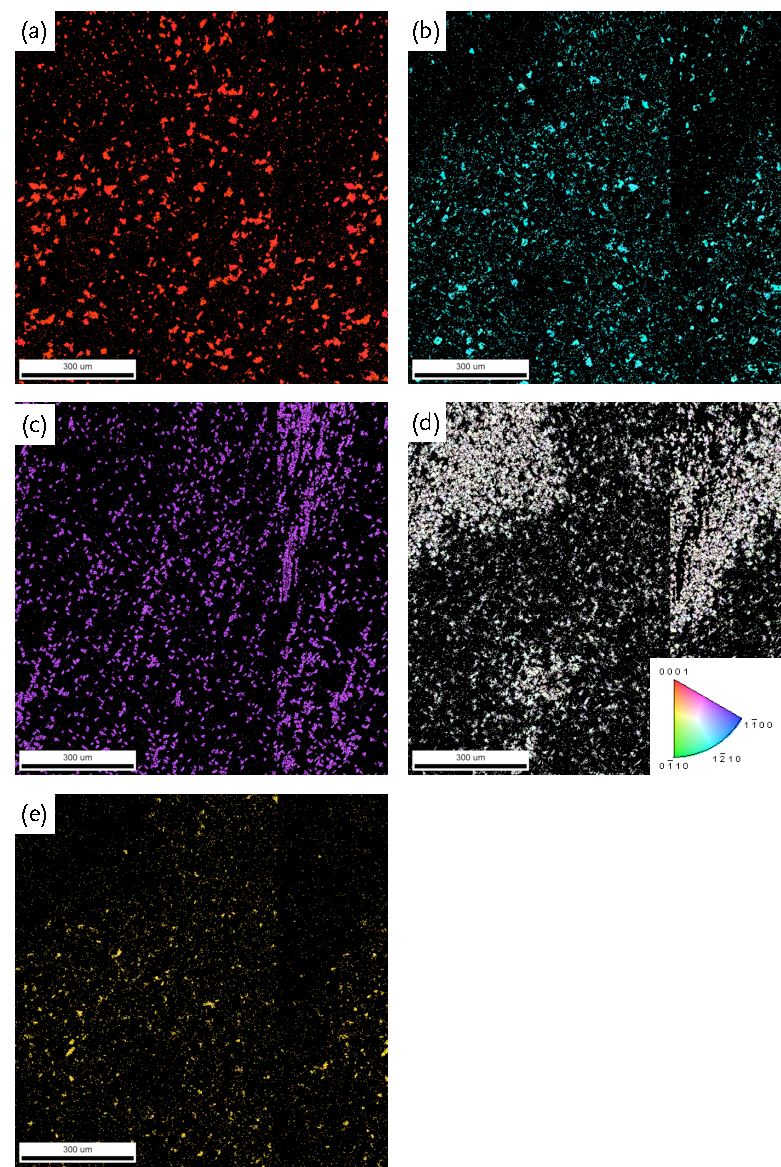
\includegraphics[width=\textwidth]{partitionmaps.pdf}
	\caption[\abbr{EBSD} figure maps for five data partitions]{%
		Pole figure maps representing the five data partitions 
		used for texture analysis. Each map is a subset of the 
		data presented in \figureref{001map}.}
	\label{fig:partitionmaps}
\end{figure}
The spacial distribution of the color bins across the scan area is nonuniform. Portions of
the scan area have a much higher distribution of grains of a certain orientation. For
example, the upper left and upper right portions of the scan area show a much higher
percentage of grains colored purple or white. At this point, it is unknown why the
distribution between the observed orientation groups is not homogeneous across the scan
surface. Possible explanations could include local temperature differences, surface
roughness differences (increased or decreased step concentration), or surface impurities.
Each of these factors could lead to different surface diffusion and nucleation rates,
causing differing nucleation and growth rates than for other areas of the sample, which in
turn affects orientation preferences.


\subsection{Pole Figure Analysis}
\label{subsec:single.growth.polefigureanalysis}


From the previous section, there are five distinct orientation relationships to determine.
The partitioned data was used to determine what these relationships are for each set of
grains. Pole figures were then generated for each of the datasets. The following is an
analysis of each set of pole figures. Unlike for the data presented for growth on
\ce{SrTiO3}(111) substrates, in this case the substrate crystal directions and sample
orientation in the microscope were tracked. For all of the following pole figures, the x-
and y-axes represent the substrate (100) and (010) directions, and the substrate (001) is
normal to the plane of the figure.


\subsubsection{Red Partition}
\label{subsubsec:single.growth.red}


%\sidefigure[Orientation analysis for red partition]{%
%	(a) Inverse pole figure for the data in the red partition. (b) Pole 
%	figure for the (0001) reflection of the red partition.
%	\label{fig:red0001}
%	}{%
%	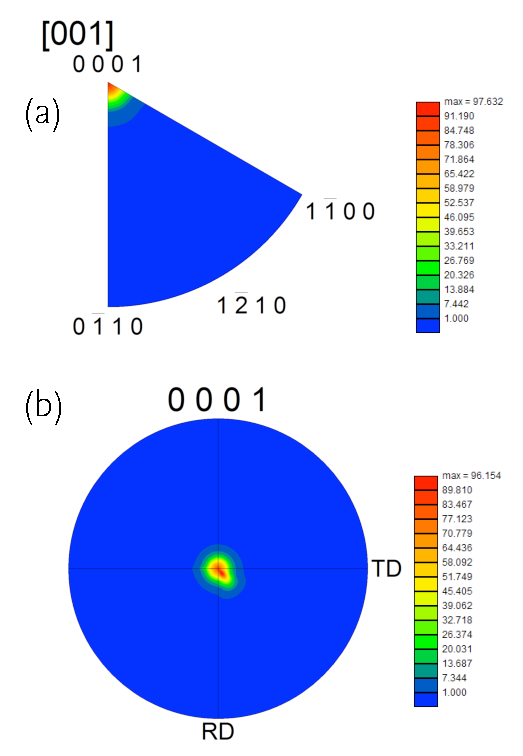
\includegraphics[width=\marginparwidth]{red0001.pdf}
%}{-5}
The partition colored red on the inverse pole map represents film grains with a c-axis
orientation. This is reflected in the inverse pole figure and (0001) pole figure found in
\figureref{red0001}. This pole figure verifies that the (0001) zone is orthogonal to the
sample surface. 
%\sidefigure[Pole figures for prismatic reflections]{%
%	Pole figures for the prismatic reflections showing 12-fold 
%	symmetry in the plane of the sample.
%	\label{fig:redinplanepole}
%	}{%
%	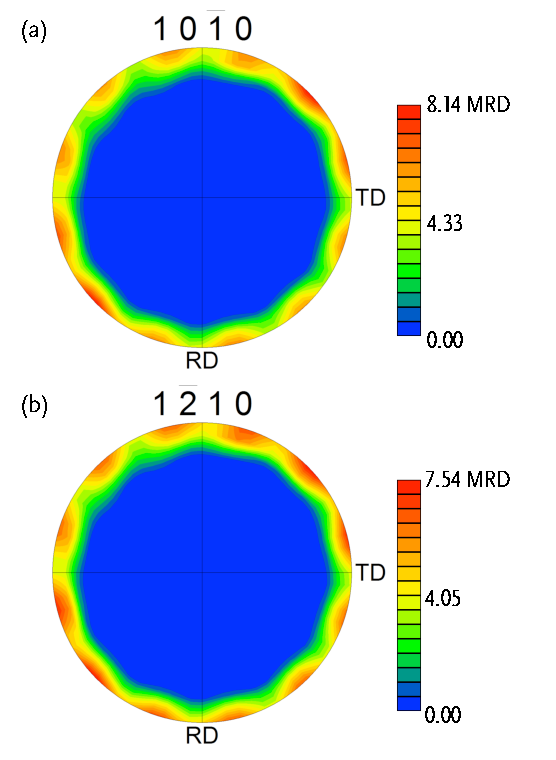
\includegraphics[width=\marginparwidth]{redinplanepole.pdf}
%}{0}
Both of these planes are perpendicular to the c-axis, and are expected to have plane
normals parallel to the sample surface. The pole figures in \figureref{redinplanepole}
verify this to be the case. Both pole figures show 12-fold symmetry, with maxima occurring
at the edge of the pole figure at regular \SI{30}{\degree} intervals. Four of the maxima
occur in alignment along the substrate <110> direction. This is consistent with the
previously observed in plane orientation relationships for growth on \ce{SrTiO3}(111)
substrates. The \ce{SrTiO3} [110] lattice distance shows 3.8\% mismatch with the
\ce{Fe2O3} a-axis lattice parameter. The (10\={1}0), (1\={1}00),  (01\={1}0) are all
crystallographically equivalent planes, separated by 60\si{\degree}. Alignment of three
equivalent film directions along four possible <110> substrate directions gives rise to
the twelve fold symmetry seen in the pole figure. The same logic extends to the (1\={2}10)
pole figure.
\begin{figure}
	\centering
	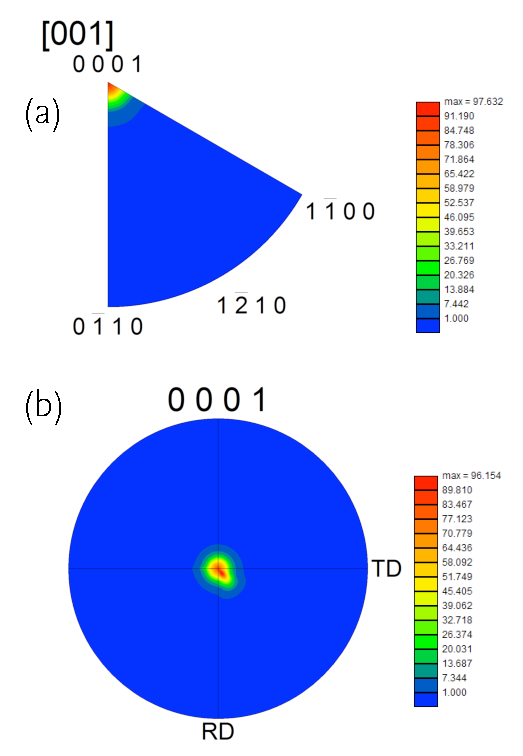
\includegraphics[width=0.5\textwidth]{red0001.pdf}
	\caption[Orientation analysis for red partition]{%
		(a) Inverse pole figure for the data in the red partition. (b) Pole 
		figure for the (0001) reflection of the red partition.}
	\label{fig:red0001}
\end{figure}
\begin{figure}
	\centering
	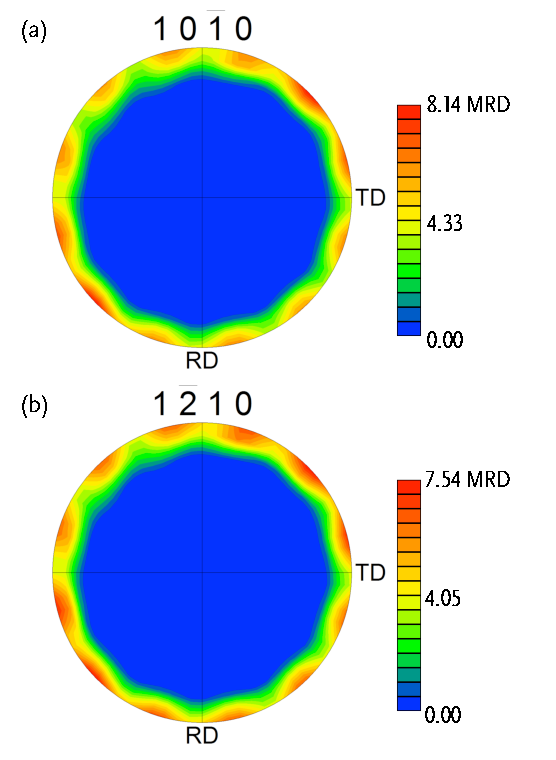
\includegraphics[width=0.5\textwidth]{redinplanepole.pdf}
	\caption[Pole figures for prismatic reflections]{%
		Pole figures for the prismatic reflections showing 12-fold 
		symmetry in the plane of the sample.}
	\label{fig:redinplanepole}
\end{figure}
For this partition, the orientation relationships can be defined as
\ce{Fe2O3}(0001)||\ce{SrTiO3}(001) and \ce{Fe2O3}(10\={1}0)||\ce{SrTiO3}(110). Equivalent
prismatic planes in the \ce{Fe2O3} crystal structure give rise to the 12-fold symmetry
observed for the (10\={1}0) and (1\={2}10) pole figures. Each of the three equivalent
<10\={1}0> directions aligns with one of the four substrate <110> directions. This
combination results in the 12-fold symmetry.


\subsubsection{Cyan Partition}
\label{subsubsec:single.growth.cyan}



%\sidefigure[Inverse pole figure for cyan partition]{%
%	Inverse pole figure for the cyan partition, representing grains with 
%	a (1\={2}10) orientation.
%	\label{fig:cyanipf}
%	}{%
%	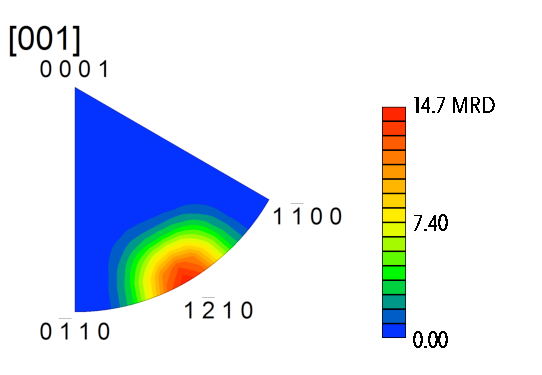
\includegraphics[width=\marginparwidth]{cyanipf.pdf}
%}{0}			
%
%
%\sidefigure[Pole figure for (0001) reflection of cyan partition]{%
%	Pole figure for the (0001) reflection of the cyan partition.
%	\label{fig:cyan0001pole}
%	}{%
%	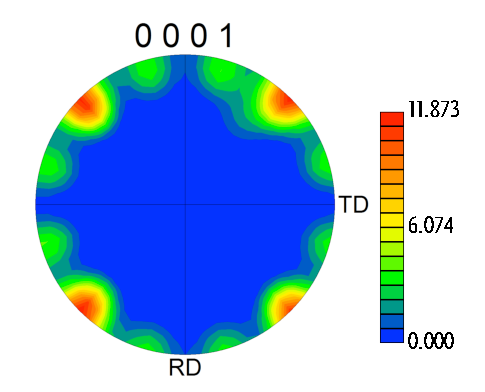
\includegraphics[width=\marginparwidth]{cyan0001pole.pdf}
%}{0}	
			
This partition represents grains near  the (1\={2}10) orientation, as shown in the inverse
pole figure depicted in \figureref{cyanall}(a). The hexagonal unit cell is aligned with
its c-axis in the plane of the sample surface. The pole figure for the (0001) plane in
\figureref{cyanall}(b) demonstrates this alignment. It shows that the (0001) zone lies in
plane, with maxima along the <110> directions, and secondary maxima spaced at 30 degree
intervals. These secondary maxima are much less intense than those along the <110> directions, roughly 3-4 \abbr{MRD} compared to a maximum of ~12 for the main peaks.
%\sidefigure[(1\={2}10) pole figure for cyan partition]{%
%	(1\={2}10) pole figure for the cyan partition. The four maxima near 
%	the substrate <111> directions were unexpected, based on the inverse 
%	pole figure.
%	\label{fig:cyan1210pole}
%	}{%
%	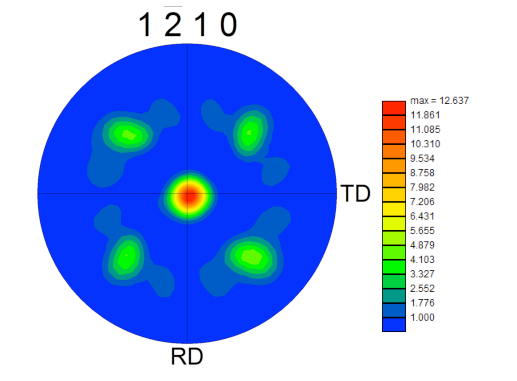
\includegraphics[width=\marginparwidth]{cyan1210pole.pdf}
%}{-3}	
Given that this partition represents points with the (1\={2}10) zone out of the surface,
it is expected that the pole figure for the (1\={2}10) reflection would show a single
maximum at the center of the pole figure. The actual pole figure, shown in
\figureref{cyanall}(c), is slightly more complicated. As expected, the most prevalent
orientation for the (1\={2}10) zone in this partition is directly out of the plane of the
sample. However four secondary maxima are observed, aligned along the <111> substrate
directions, tilted ~57\si{\degree} away from the sample normal direction. This orientation
is explored in more detail for the purple and white partitions, which both share this
alignment of the film c-axis with a substrate <111> direction.
\begin{figure}
	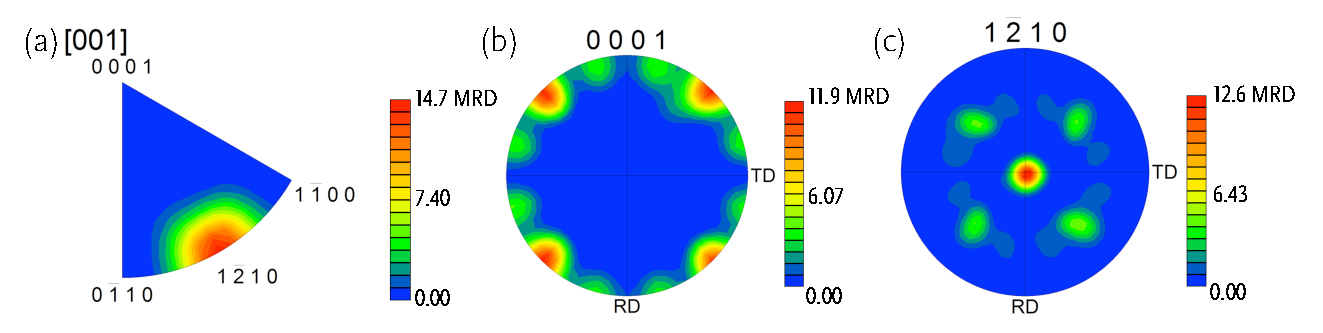
\includegraphics[width=\textwidth]{cyanall.pdf}
		\caption[Pole figure for cyan partition]{%
			(a) Inverse pole figure for the cyan partition, representing grains with 
	a (1\={2}10) orientation. (b) Pole figure for the (0001) reflection of the cyan
partition. (c) (1\={2}10) pole figure for the cyan partition. The four maxima near 
	the substrate <111> directions were unexpected, based on the inverse 
	pole figure.}
	\label{fig:cyanall}
\end{figure}
The reasons for the c-axis alignment along the (110) direction, and for the (1\={2}10)
peaks along the substrate (111) directions are not yet understood. It is possible that 
during the binning of the original dataset, a certain subset of points falling between the 
white bin and the cyan bin were included in the latter group, resulting in the secondary 
peaks shown here. The orientation relationships are \ce{Fe2O3}(0001)||\ce{SrTiO3}(110) and
\ce{Fe2O3}(1\={2}10)||\ce{SrTiO3}(001).


\subsubsection{Purple and White Partitions}
\label{subsubsec:single.growth.purplewhite}

\begin{figure}
	\begin{center}
		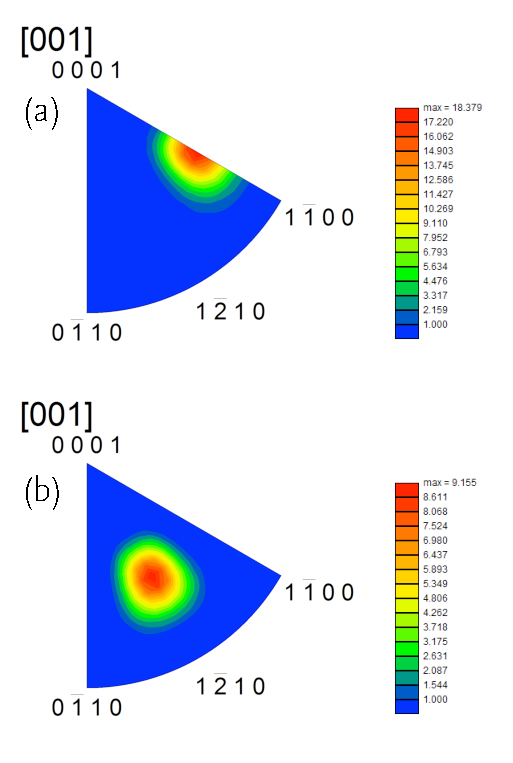
\includegraphics[width=0.5\textwidth]{purplewhiteipf.pdf}
		\caption[Inverse pole figures for purple and white grains]{%
         	Inverse pole figures showing (a) the (1\={1}02) orientation of the purple 
         	grains and (b) the (1\={2}13) orientation of the white grains.}
		\label{fig:purplewhiteipf}
	\end{center}
\end{figure}
%\sidefigure[Inverse pole figures for purple and white grains]{%
%	Inverse pole figures showing the (1\={1}02) orientation of the purple 
%	grains (a) and the (1\={2}13) orientation of the white grains (b)
%	\label{fig:purplewhiteipf}
%	}{%
%	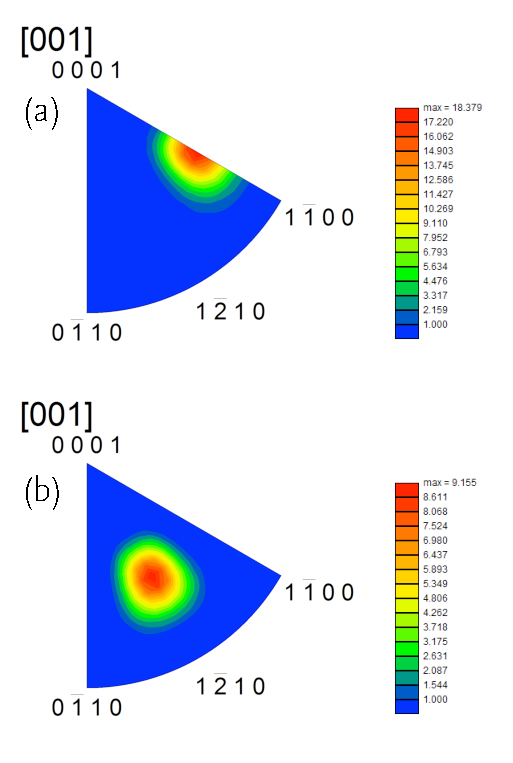
\includegraphics[width=\marginparwidth]{purplewhiteipf.pdf}
%}{-2}				
The white and purple partitions represent the most interesting orientation relationship
between the film grains and the substrate. These partitions represent grains with
(1\={1}02) and (1\={2}13) orientations respectively. Inverse pole figures verifying these
orientations are shown in \figureref{purplewhiteipf}. The inverse pole figures suggest
that both of these orientations represent grains that have a c-axis tilted roughly the
same angle away from normal to the sample surface. The surface orientation differs by a
rotation around this tilted c-axis.
\begin{figure}
\begin{center}
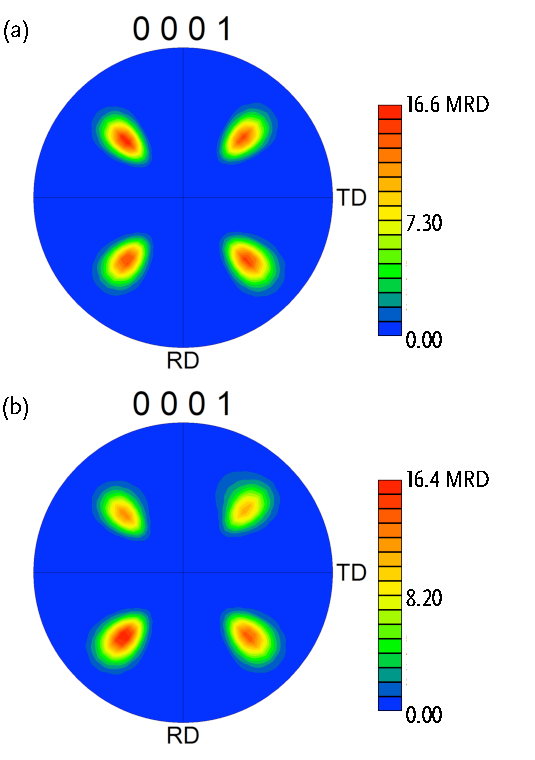
\includegraphics[width=0.5\textwidth]{purplewhite0001pole.pdf}
\caption[(0001) pole figures for purple and white grains]{%
	Pole figures for the (0001) reflection for the purple partition (a) 
	and the white partition (b). The (0001) zone is located directly in 
	line with the substrate <111> directions.}
\label{fig:purplewhite0001pole}
\end{center}
\end{figure}
%\sidefigure[(0001) pole figures for purple and white grains]{%
%	Pole figures for the (0001) reflection for the purple partition (a) 
%	and the white partition (b). The (0001) zone is located directly in 
%	line with the substrate <111> directions.
%	\label{fig:purplewhite0001pole}
%	}{%
%	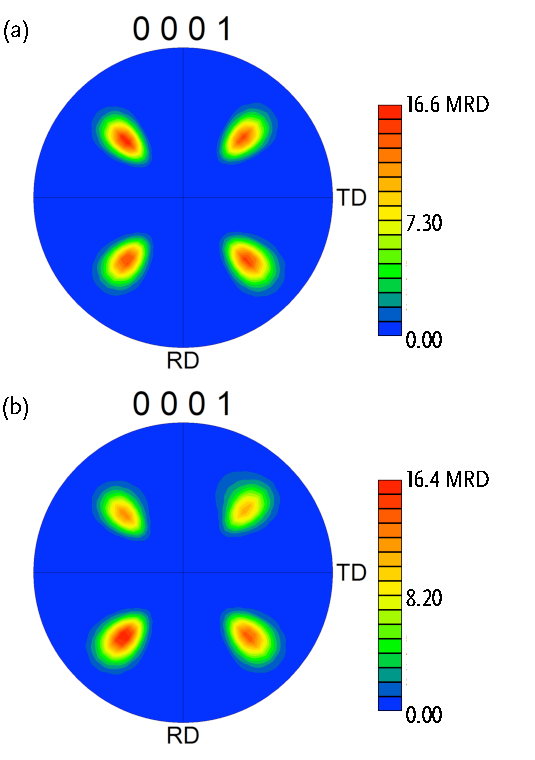
\includegraphics[width=\marginparwidth]{purplewhite0001pole.pdf}
%}{8}	
Pole figures for the (0001) planes for these partitions are shown in
\figureref{purplewhite0001pole}. Both pole figures show the same orientation preference
for the (0001) reflection. Four maxima are observed, located ~57-60\si{\degree} from the
center of the pole figure. The four maxima are observed in line with the (111) cubic
substrate directions. The substrate (111) direction is located 54.7\si{\degree} away from
the out of plane (001) direction. The angle between the (0001) and (1\={1}02) planes for
the \ce{Fe2O3} film is 57.6\si{\degree}, and the angle between the (0001) and (1\={2}13)
directions is 61\si{\degree}. If the orientation relationship for these film grains and
the substrate is driven by the alignment of the substrate (111) direction with the film
(0001) direction, this would lead to (1\={2}13) and (1\={1}02) planes parallel to the
sample surface, as observed in the inverse pole figure. 

For these grains, the orientation relationship can be summarized with the relation
\ce{Fe2O3}(0001)||\ce{SrTiO3}(111).  This is the same relationship determined for films on
\ce{SrTiO3}(111) substrates. However in that case, the (111) direction was directly out of
the plane of the sample, and an in plane direction with low lattice mismatch was
identified to explain the in plane alignment. In this case, the 2-D lattice parameters at
the sample surface don't appear to be the driving force for the film's orientation
relationship. Instead, substrate directions drive the relationship. More vectors than just
the substrate and film normal and in plane directions must be taken into account to
predict the structure of the film. The same epitaxial relationship of the film c-axis
aligning with the substrate (111) direction, even when that substrate direction is tilted
to high angles away from the surface.

In some ways, this is similar to the idea of axiotaxial film growth. Axiotaxy is defined
as a fiber-like film growth mode, with a film direction aligning along a substrate
direction, though not necessarily the substrate direction orthogonal to the substrate
surface. In both axiotaxy and the purple and white partitions of the films reported here,
crystal directions appear as the dominant driver of orientation relationship, rather than
lattice match between the substrate and the film. However, axiotaxial growth exhibits a
rotational degree of freedom around the film growth axis.  If these partitions showed true
axiotaxial growth, the pole figures for the prismatic planes of the film would be expected
to show circular patterns around the rotation axis. This is not the case.
\figureref{purplewhiteprismatic} shows pole figures for the prismatic (1\={2}10) and
(10\={1}0) planes.
\begin{figure}
	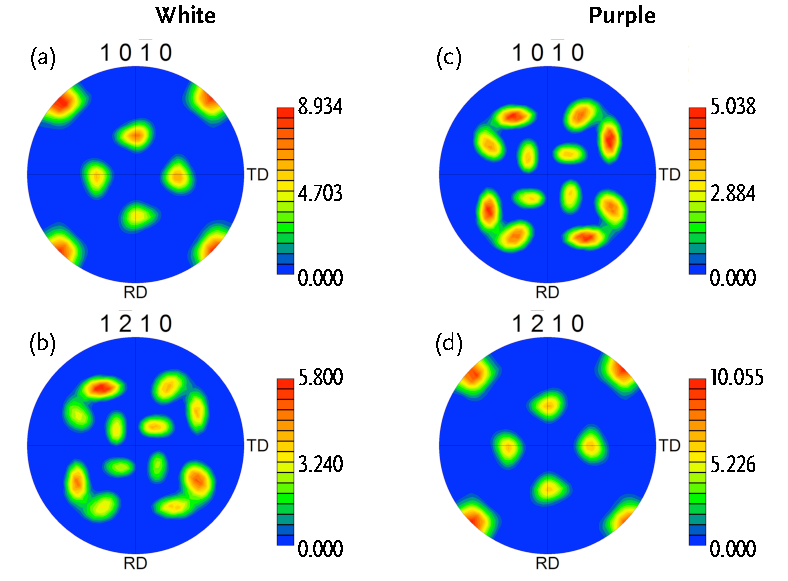
\includegraphics[width=\textwidth]{purplewhiteprismatic.pdf}
	\caption[Prismatic pole figures for white and purple grains]{%
		Pole figure for the prismatic zones of the white and purple partitions. 
		These pole figures suggest a three fold rotation around the film c-axis 
		(which is aligned along the substrate [111] direction, as seen in 
		\figureref{purplewhite0001pole}).}
	\label{fig:purplewhiteprismatic}
\end{figure}
Instead of circular bands, these faces demonstrate 3-fold symmetry when rotated around the
film (0001) direction. In the case of the white partition, the (10\={1}0) film direction
appears to line up with the substrate (110) directions. For the purple partition, the
substrate (110) direction lines up with the film (1\={2}10) direction. The maxima along
the rolling direction (RD) and the transverse direction (TD) in these pole figures are
located 45\si{\degree} away from the center of the figure. This supports the idea that
these maxima are in line with the (011) directions. 

For all data represented in these pole figures, the orientation relation
\ce{Fe2O3}(0001)||\ce{SrTiO3}(111) holds true. For the white partition, that is, grains
with the direction normal to the film (1\={2}13) plane normal to the surface, the
(10\={1}0) planes are in line with the substrate (110) planes. For the purple partition,
grains with a (1\={1}02) orientation, the (1\={2}10) planes are in line with the substrate
(110) planes. 


\subsubsection{Yellow Partition}
\label{subsubsec:single.growth.yellow}

\begin{figure}
\centering
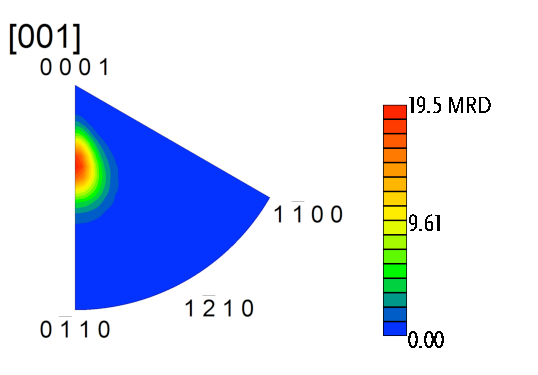
\includegraphics[width=0.5\textwidth]{yellowipf.pdf}
\caption[Inverse pole figure showing orientation of  yellow grains]{%
Inverse pole figure showing the (01\={1}4) orientation of yellow grains.}
\label{fig:yellowipf}

\end{figure}
%\sidefigure[Inverse pole figure showing orientation of  yellow grains]{%
%	Inverse pole figure showing the (01\={1}4) orientation of yellow grains.
%	\label{fig:yellowipf}
%	}{%
%	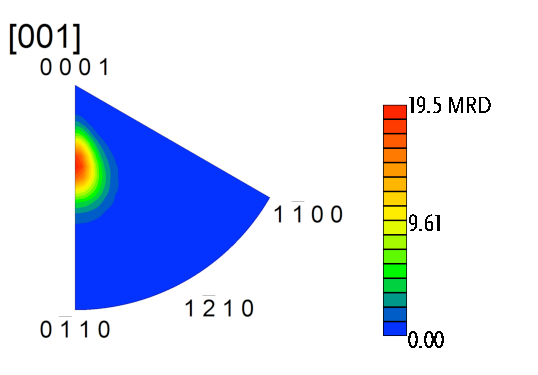
\includegraphics[width=\marginparwidth]{yellowipf.pdf}
%}{-8}		
The final partition of this dataset is not yet understood. The yellow partition represents
a significantly smaller portion of the original scan than the other datasets, and doesn't
lend itself to easy interpretation either through lattice mismatch or an analysis of
c-axis tilt angles, as were used for previous orientation relationship determination. This
partition represents (01\={1}4) oriented grains, as determined from the inverse pole
figure and (01\={1}4) pole figure shown in Figures \ref{fig:yellowipf} and
\ref{fig:yellow0114pole}.

\begin{figure}
\begin{center}
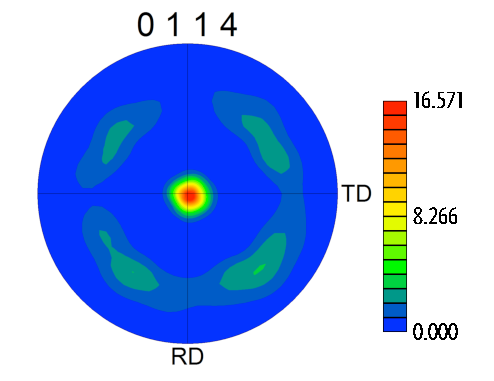
\includegraphics[width=0.5\textwidth]{yellow0114pole.pdf}
\caption[(01\={1}4) pole figure for yellow grains]{%
	Pole figure for the (01\={1}4) reflection of the (01\={1}4)-oriented yellow
partition.}
\label{fig:yellow0114pole}
\end{center}
\end{figure}
%\sidefigure[(01\={1}4) pole figure for yellow grains]{%
%	Pole figure for the (01\={1}4) reflection of the (01\={1}4)-oriented yellow
%partition.
%	\label{fig:yellow0114pole}
%	}{%
%	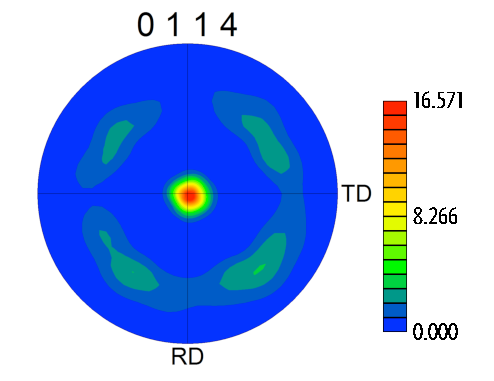
\includegraphics[width=\marginparwidth]{yellow0114pole.pdf}
%}{-5}	
			
\begin{figure}
\begin{center}
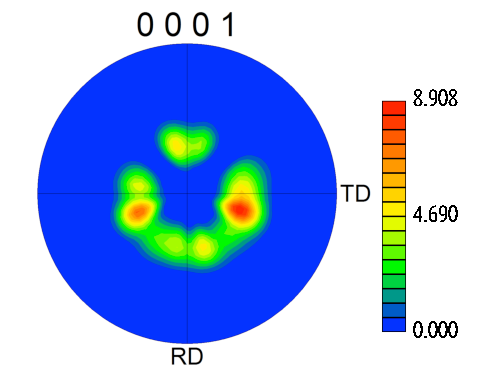
\includegraphics[width=0.5\textwidth]{yellow0001pole.pdf}
\caption[(0001) pole figure for yellow grains]{%
	Pole figure for the (0001) reflection of the yellow partition.}
\label{fig:yellow0001pole}
\end{center}
\end{figure}
%\sidefigure[(0001) pole figure for yellow grains]{%
%	Pole figure for the (0001) reflection of the yellow partition.
%	\label{fig:yellow0001pole}
%	}{%
%	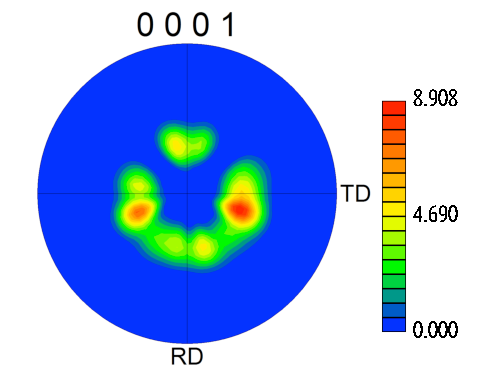
\includegraphics[width=\marginparwidth]{yellow0001pole.pdf}
%}{7}				
\figureref{yellow0001pole} shows a pole figure for the (0001) plane. The maxima for this
pole figure are less easily understood.  The pole doesn't show the same qualities seen in
the previous figures; the (0001) zone isn't located in alignment with easily identified
low-index substrate directions, and doesn't show the 4-fold or 12-fold symmetry seen in
previous cases. The maxima in the southern hemisphere of the pole figure do suggest the
beginnings of twelve fold symmetry. The lack of highly evident maxima corresponding to the
remaining points of the 12-fold rotation could be a result of the small size of this
dataset. The low number of points could mean that this pole figure shows an incomplete
picture, and more scan data would fill in the rest of the symmetry. Two peaks, colored red 
and located just below the horizontal axis, are significantly stronger than the remainder, 
and suggest a possible starting point for future examination. From the inverse pole figure 
in \figureref{yellowipf}, the orientation relationship 
between the substrate and film normal is \ce{Fe2O3}(01\={1}4)||\ce{SrTiO3}(001). The in
plane relationship is not yet determined. At this point no clear explanation for the 
nucleation of (01\={1}4) oriented film grains has been discovered.


\subsection{Discussion}
\label{subsec:single.growth.discussion}

For each orientation group,\footnote{With the exception of the yellow grains, for which a
clear orientation relationship could not be determined.} the orientation relationship was
determined. In some cases the same alignment of a vector or plane was found, even though
the out of plane orientation differed. For example, the cyan, white, and purple
orientations all share the relationship \ce{Fe2O3}[10\={1}0]||\ce{SrTiO3}[1\={1}0]. The
purple and white orientations both have their (0001) planes parallel to the substrate
(111) planes.

An interesting way to understand the observed epitaxial relationships is to consider the
arrangement of close-packed (eutactic)\cite{OKeeffe:1977vx}
networks.\footnote{\chapterref{polycrystalline.growth} also discusses \ce{Fe2O3} thin film
growth and the concept of eutactic arrangements in the context of growth on high index
surfaces of polycrystalline substrates.} The hematite structure is a hexagonal close
packed (hcp) network of oxygen atoms, with iron atoms filling \slantfrac{2}{3} of the
interstitial sites. The close packed oxygen plane is the (0001) plane, and the close
packed direction within this plane is the <1\={1}00> family of directions. The \ce{SrTiO3}
substrate is a cubic close packed (ccp) network of \ce{SrO3} atoms, with titanium atoms in
\slantfrac{1}{4}{ of} the octahedral interstitial sites. The close packed planes are the
\{111\} family of planes, and the close packed directions within that plane are <1\={1}0>.


Each orientation group is represented by the alignment of one or both of the close packed
plane or close packed direction between film and substrate. The white partition, oriented
at (1\={2}13), represent grains with both the close packed planes and directions forming
the orientation relationships. In this partition, the  (0001) planes of the film is
parallel to the substrate (111) planes. The film [10\={1}0] film direction is parallel to
the substrate [1\={1}0] direction. This orientation represents a continuation of the
eutactic network between the substrate and film.

Other partitions have at least one close packed alignment. The cyan orientation represents
the alignment of the close packed directions. The red orientation also matches the close
packed direction. The purple orientation shares the alignment of the close packed planes
exhibited by the white partition, but the close packed directions are not aligned.
Instead, the close packed direction of the film is rotated \texttildelow30\degree{} from
the substrate close packed direction.

These results suggest that an analysis of the eutactic network can provide a useful guide
for the prediction and analysis of film textures, especially in the case of heteroepitaxy
with poor lattice parameter matching. In this case, it is difficult to find an
arrangement for the hexagonal film that matches well with the cubic substrate. Instead, those
close packed network suggests the alignments seen in these results.


\section{Conclusions}
\label{sec:single.growth.conclusions}


Hematite \ce{Fe2O3} films were grown on single crystal \ce{SrTiO3} substrates. On (111)
oriented substrates, the orientation relationships between film and substrates were
determined to be \ce{Fe2O3}(0001)||\ce{SrTiO3}(111) and
\ce{Fe2O3}(10\={1}0)||\ce{SrTiO3}(1\={1}0). Polycrystalline films grew on (001) oriented
substrates. The film grains showed preferred orientations, falling into five orientation
groups. A portion grains were (0001) oriented, a second group was oriented with the (0001)
zone parallel to the sample surface, and a portion retained the
\ce{Fe2O3}(0001)||\ce{SrTiO3}(111) relationship, despite the (001) orientation of the
substrate.